\documentclass{article}

\usepackage{amsmath}
\usepackage{amssymb}
\usepackage{mathtools}
\usepackage{fullpage}
\usepackage{enumerate}
\usepackage{graphicx}

\title{Computer Science 577 Notes \\ Introduction to Algorithms}
\author{Mendel C. Mayr}
\date{\today}

\begin{document}
	\maketitle
	\vspace{10pt}
	\begin{center}
		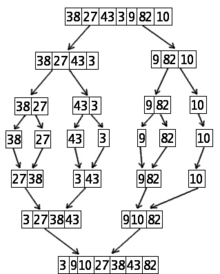
\includegraphics[width = 2.7in]{mergesort.png}
		\end{center}
	\vspace{12pt}
	\tableofcontents
	\clearpage

	\section{Recurrence Relations}
		\subsection{Recursive Analysis of Insertion and Merge Sort}
			Insertion sort: let $M(n)$ be the comparisons required to sort a list of size $n$ \\
			Analysis: note that $M(1) = 0$ and $M(n) = M(n - 1) + n$ for $n > 1$
			\begin{enumerate}[(i)]
				\item $M(n) = M(n - 1) + n$
				\item $M(n) = M(n - 2) + n + (n - 1)\:...$
				\item $M(n) = M(n - k) + n + (n - 1) +\:...\:+ (n - k + 1)$
				\item Let $k = n - 1$, $M(n) = M(1) + n(n - n + 1) + \sum_{i = 1}^{n - 1}i$
				\item $M(n) = 0 + n + (n - 1)(n - 2)/2 \approx n^2/2$
				\end{enumerate}
			Merge sort: let $M(n)$ be the comparison required to sort a list of size $n$ \\
			\\
			Analysis: for simplcity, consider only $n$ such that $n = 2^a$ for some integer $a$ \\
			Note that $M(1) = 0$ and $M(n) = 2M(n/2) + n$ for $n > 1$
			\begin{enumerate}[(i)]
			 	\item $M(n) = 2M(n/2) + n$
			 	\item $M(n) = 2M(n/4) + n + (n/2)$
			 	\item $M(n) = 2M(n/2^k) + n + (n/2) +\:....\:+ (n/2^{k - 1})$
			 	\item Let $k = a$, $2M(1) + \sum_{i = 1}^{k - 1} n/2^i$ (unclarified point)
			 	\item Mergesort is $O(n \log n)$
			 	\end{enumerate}
		\subsection{Recursive Linear Selection}
			Recursive linear selection algorithm: given $x_1, x_2, ..., x_n$ distinct keys, find $x_k$ (i.e. the $k$th smallest element) without using sorting \\
			Note: the rank of an element (i.e. the number of keys greater than it) can be found in linear time \\
			Linear selection algorithm is as folows:
			\begin{enumerate}[(i)]
				\item Remove keys of known rank, to make $n = 5 (mod 10)$
				\item Divide elements into groups of 5, denoted $S[i]$ for $i$ from $1$ to $n/5$
				\item Recursively find the median of each group, denoted $x[i]$
				\item Let $M^*$ be the median of the set $x[i]$ for $i$ from $1$ to $n/5$
				\item Divide keys into groups of keys less than (call this $L$), equal to, or greater than (call this $R$) $M^*$
				\item Recursiveley process one of $L$ or $R$
				\end{enumerate}
			Analysis: Note that steps 1, 2, and 5 are $O(n)$, so the number of computations for this algorithm, $T(n) = T(n/5) + T(7n/10) + O(n)$ \\
			Guessing and proving: supposed that $T(n) = O(n)$, which can be proven via strong induction, i.e. $T(n) < An$ for some constant $A$ for all $n$ \\
			Recall that strong induction relies on proving two claims:
			\begin{enumerate}[(i)]
				\item The statement holds for all $n \geq 1$, $\forall n \leq n_0$ (base case)
				\item If the statmenet holds for all $i < n$, it holds for $n$
				\end{enumerate}
			Proof of second part of strong inductive proof:
			\begin{enumerate}[(i)]
				\item Suppose that $T(n) = O(n)$ for $i < n$
				\item We seek and $A$ such that $A(n/5) + A(7n/10) + cn \leq An$
				\item Thus, $A \geq 10c$ is sufficient for this part
				\end{enumerate}
			Proof of first part of strong inductive proof: need $A$ such that $n(n - 1)/2 \leq An$ for $1 \leq n \leq 10$ \\
			So $A \geq 9/10$ is sufficient for this part \\
			\\
			Conclusion: $A = max\{9/2, 10c\}$ will suffice to show that $T(n) = O(n)$ 
		\subsection{Recursive Quadratic Closest-Pair}
			Recursive quadratic algorithm: find closest pair of points
			\begin{enumerate}[i]
				\item (Supposing that $n = 2^k$) into 2 equal groups, denoted $L$ and $R$
				\item Recurisvely find the closest pair in $L$ and $R$
				\item Report closest pair form testing elements of $L$ against elements of $R$
				\item Report best pair out of those from steps (ii) and (iii)
				\end{enumerate}
			Analysis: $T(n) = 2(T/n) + O(n^2)$ for $n = 2^k \geq 4$, $T(2) = 1$ \\
			The $O(n^2)$ in the recursive case comes from step (iii) \\
			\\
			Consider the recursion tree, which is full binary tree: at the first level, the problem size is $n, n/2, n/4, ...$ at the first, second, third, etc. levels. Thus, the number of computations required is $n^2$ at the first level, $2(n/2)^2 = n^2/2$ at the second level, $2(n/4)^2 = n^2/4$ at the third, etc. \\
			\\
			Thus, the maximum number of computations is $\sum_{k = 1}^\infty n^2/2^k = 2n^2$, thus $T(n) = O(n^2)$
		\subsection{Divide and Conquer Recurrences and Master Theorem}
			Master theorem: if $T(n) = aT(n/b) + O(n^d)$ for some constants $a > 0, b > 1$, and $d \geq 0$, then:
			\begin{enumerate}[(i)]
				\item $T(n) = O(n^d)$ if $d > \log_b a$
				\item $T(n) = O(n^d \log n)$ if $d = \log_b a$
				\item $T(n) = O(n^{\log_b a})$ if $d < \log_b a$
				\end{enumerate}
			Proof: consider the recursion tree for such a problem \\
			Notice that $a$ is the branching factor of the problem. At the $i$th level (starting at index 0), there are $a^i$ subproblems of size $n/b^i$. which means the computation that must be done at that level is $a^iO((n/b^i)^d)$ \\
			The number of levels in the recusion tree is $k = \log_b n$ \\
			As such: $T(n) = \sum_{i = 0}^k a_iO((n/b^i)^d) = O(n^d)\sum_{i = 0}^k(a/b^d)^i$. Now consider the cases
			\begin{enumerate}[(i)]
				\item If $d > \log_b a$, then $a/b^d < 1$ \\
				$\sum_{i = 0}^\infty (a/b^d)^i < \infty$ (i.e. series converges) \\
				$\sum_{i = 0}^\infty (a/b^d)^i = O(1)$, so $T(n) = O(n^d)$
				\item If $d = \log_b a$, then $a/b^d = 1$ \\
				$\sum_{i = 0}^k (a/b^d)^i = \sum_{i = 0}^k 1 = k + 1$, since $k = \log_b n = \log n/\log b = O(\log n)$ \\
				Therefore, $T(n) = O(n^d\log n)$
				\item If $d < \log_b a$, then $a/b^d > 1$ \\
				$\sum_{i = 0}^k (a/b^d)^i = O((a/b^d)^k)$, so $T(n) = O(n^d)O(a^k)/b^{dk}$ \\
				Since $k = \log_b n, n = b^k$, $T(n) = O(n^d)O(a^k)/n^d = O(a^k)$ \\
				$a^k = a^{\log_b n} = n^{\log_b a}$, so $T(n) = O(n^{\log_b a})$
				\end{enumerate}
		\subsection{Asymptotics}
			Notation for asymptotics:
			\begin{enumerate}[(i)]
				\item $f$ and $g$ are real value functions on $x \geq 0$. $f(x)$, $g(x) \geq 0$ for sufficiently large $x$ \\
				Sufficently large: $\exists x_0 > 0$ such that $f(x) \geq 0$ when $x \geq x_0$
				\item $f = O(g)$ means that for some $c > 0$ and $x_0 > 0$, $f(x) \leq cg(x)$ for al $x \geq x_0$
				\item $f = \Omega(g)$ means that for some $c > 0$ and $x_0 \geq 0$, $f(x) \geq xg(x)$ for all $x \geq x_0$ \\
				This is equivalent to saying that $g = O(f)$
				\item $f = \Theta(g)$ means that $f = O(g)$ and $f = \Theta(g)$
				\end{enumerate}
			Demonstrating that $f = O(g)$ can be done algebraically, or via L'Hopital's rule \\
			\\
			Additional definitions:
			\begin{enumerate}[(i)]
				\item $f = o(g)$ means $\lim_{x \to \infty} f(x)/g(x) = 0$
				\item $f \sim g$ means $\lim_{x \to \infty} f(x)/g(x) = 1$
				\end{enumerate}
			Polynomial growth: $f$ is polynomially bounded if $f(x) = O(x^k)$ for some $k > 0$, (efficiently computable) \\
			Exponential growth: $f$ is exponential growth if $f(x) = O(\alpha^x)$ for some $\alpha > 1$
		\clearpage

	\section{Arithmetic Algorithms and Sorted Lists}
		\subsection{Arithmetic Algorithms}
			Addition: elementary (i.e. sum and carry bits), adding two $n$-bit numbers has $O(n)$ complexity \\
			Subtraction: inverse of addition, similarly requires $O(n)$ times \\
			Multiplication: elementary algorithm requires $O(n)$ times
			\\
			There exists an $O(n^a)$ algorithm for multiplication, where $a < 2$: \\
			For multiplying $n$-bit numbers, where $n = 2^k$:
			\begin{enumerate}[(i)]
				\item $x = 2^{n/2}x_1 + x_0$, $y = 2^{n/2}y_1 + y_0$
				\item $xy = 2^nx_1y_1 + 2^{n/2}(x_1y_0 + x_0y_1) + x_0y_0$
				\item Let $a = x_1y_1$, $c = x_0y_0$, $d = (x_1 + x_2)(y_1 + y_2)$
				\item Let $b = x_1y_0 + x_oy_1$, note that $b = D - A - C$
				\end{enumerate}
			Analysis: let $k(n)$ be the complexity of this algorithm \\
			$k(n) = 3k(n/2) + O(n)$ when $n > 1$, $K(n) = O(1)$ when $n = 1$ \\
			By the master theorem: $k(n) = O(n^{\log_2 3}) \approx O(n^{1.59})$ \\
			\\
			Using Newton interation, division reducible to multiplication: similar complexity \\
			Open question: does there exist $O(n)$ algorithm for multiplication \\
			\\
			Matrix multiplication: let $A = (a_{i, j}), B = (b_{i ,j})$ for $1 \leq i, j \leq n$ \\
			Then $C = (c_{i, j})$, where $c_{i, j} = \sum_{k = 1}^n a_{i, k}n_{k, j}$ \\
			Recursive algorithm for matrix multiplication: subblocks of matricies can be multipled as follows
			\begin{equation*}
				\text{Since } X = \begin{bmatrix} A & B \\ C & D \end{bmatrix}
				\text{ and } Y = \begin{bmatrix} E & F \\ G & H \end{bmatrix}
				\text{, then } XY = \begin{bmatrix}	AE + BG & CE + DG \\ AF + BH & CF + DH \end{bmatrix}
				\end{equation*}
			The 8 products required tocan be found recursively, resulting in $T(n) = 8T(n/2) + O(n^2) = O(n^3)$ \\
			A matrix decomposition can be used to make a faster algorithm, requiring only 7 products:
			\begin{equation*}
				\begin{bmatrix}
					P_5 + P_4 - P_2 + P_6 & P_1 + P_2 \\
					P_3 + P_4 & P_1 + P_5 - P_3 - P_7
					\end{bmatrix}
				\end{equation*}
			The products $P_1, P_2, ..., P_7$ are defined respectively as: \\
			$A(F - H), (A + B)H, (C + D)E, D(G - E), (A + D)(E + H), (B - D)(G + H), (A - C)(E + F)$ \\
			The complexity, by the master theorem, is: $T(n) = 7T(n/2) + O(n^2) = O(n^{\log_2 7}) \approx O(n^{2.81})$
		\subsection{Quicksort}
			Quicksort algorithm: given array $E$
			\begin{enumerate}[(i)]
				\item Selects pivot element, moves element to local variable
				\item Partition subroutine rearranges elements about a $splitPoint$ such that:
				\begin{enumerate}[(a)]
					\item For $first \leq i < splitPoint$, $E[i] < pivot$
					\item For $splitPoint < i \leq last$, $E[i] \geq pivot$
					\end{enumerate}
				\item Pivot element goes in $E[splitPoint]$
				\item Recursively sort the smaler and larger subarrays
				\end{enumerate}
			Analysis of quicksort: \\
			Worst case: already sorted in ascending order, smallest element selected as pivot \\
			Complexity in worst case is: $\sum_{k = 2}^n(k - 1) = n(n - 1)/2$ \\
			\\
			Average behavior: suppose all permutations of keys are equally likely
			\begin{enumerate}[(i)]
				\item For an array of size $k$, partition does $k - 1$ key comparisons \\
				Subranges have $i$ and $k - 1 - i$ elements each
				\item This gives the following recurrence: $A(n) = 0$ for $n = 1$ or $n = 2$ \\
				$A(n) = n - 1 + \sum_{i = 0}^{n - 1} (1/n)(A_i) + A(n - 1 - i)$ for $n \geq 2$ \\
				Which is that same as: $A(n) = n - 1 + (2/n)\sum_{i = 1}^{n - 1} A(i)$ for $n \geq 1$
				\item A good case for quicksort is if each partition divides the array into 2 arrays of size $n/2$ each \\
				In this case: $Q(n) \approx n + 2Q(n/2)$, so by the master theorem $Q(n) = \Theta(n \log{n})$
				\end{enumerate}
			Theorem: let $A(n)$ be defined by the recurrence as above. Then for $n \geq 1$, $A(n) \leq cn\ln(n)$ for some constant $c$ \\
			\\
			Proof: strong induction supposes that $A(i) \leq ci\ln(i)$ for $1 \leq i < n$ \\
			Thus, suppose that $A(n) \leq n - 1 + (2/n)\sum_{i = 1}^{n - 1} ci \ln(i)$ \\
			$A(n) \leq n - 1 + (2/n)\int_1^n x \ln(x) dx = cn\ln(n) + n(1 - c/2) - 1$ \\
			Let $c = 2$ so that $A(n) \leq 2 n\ln(n)$. A similar analysis shows that $A(n) > cn\ln(n)$ for $c < 2$ \\
			\\
			Corrolary: average case of number of comparisons done by quicksort is $1.386n\log(n)$ for large $n$
		\subsection{Random Choices in Algorithms}
			Example: seearch aray for a 1, where $\Sigma = \{0, 1\}$, and array has $50\%$ 0s \\
			A deterministic algorithm will use a linear search, with worst case taking $n/2$ time \\
			Let $T$ be the queries to find: $E(T) = \sum_{t = 0}^\infty t/2^t = 2$ \\
			\\
			Example: Quicksort (with randomly chosen pivot) to sort distinct set $x_1, ..., x_n$ \\
			Choose $1 \leq i \leq n$ at random, let pivot $p = x_i$ \\
			Acts just like quicksort on a randomly ordered input \\
			\\
			Skip lists: storing a list of distinct sorted numbers \\
			Multilevel indicies, i.e. various elements stored in nodes, with 2-way connections between:
			\begin{enumerate}[(i)]
				\item Adjacent elements (connections between elements of the same level)
				\item Identical elements (connections between various levels)
				\end{enumerate}
			Tab locations (e.g. nodes at higher levels) made using random choices \\
			Setinels: use before and after at each level (e.g. $\infty$ and $-\infty$) \\
			To find value: start at highest level, decend right before element value is passed \\
			\\
			The number of levels for any particular index is randomly determined \\
			Number of nodes in skip list: $E(\#nodes) = \sum_{x \in keys}E(height)$, where $E(height) = 2$ \\
			The height of the skip list is based on a geometric random variable, i.e. height is flip number for first head \\
			Analysis of skip lists: expected cost of search, insert, and delete is $O(\log{n})$
		\subsection{Splay Trees}
			Amortized analysis: expected complexity value for a series of operations \\
			Splaying: used to create logarithmic amortized bound \\
			\\
			Splaying restructures tree to move latest node to the root
			\begin{enumerate}[(a)]
				\item Zig case: single rotation to put $x$ at root
				\item Zig-zag case: two single rotations, parent and grandparent each rotated
				\item Zig-zig case: double rotation, parent and grandparent rotated at once via $x$
				\end{enumerate}
			\begin{center}
				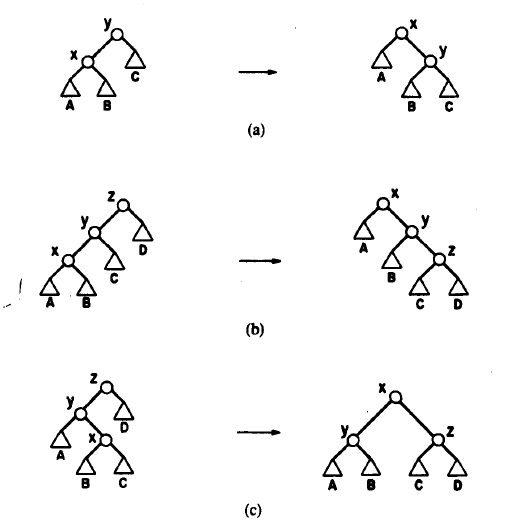
\includegraphics[width = 2.7in]{splaying.png}
				\end{center}
			Triangles in figure represent subtrees. Trees shown here can themselves be subtrees \\
			\\
			Operations on splay trees: element $x$
			\begin{enumerate}[(i)]
				\item Insertion: splay upon insertion, $x$ becomes new root
				\item Find: if search is successful, splay $x$ to new root, otherwise, last node access prior to reaching null value becomes new root
				\item FindMin and FindMax: splay after access, $x$ moved to root
				\item DeleteMin and DeleteMax:
				\begin{enumerate}[(a)]
					\item DeleteMin: perform FindMin, brining minimum to root \\
					By binary search tree property, no left child. Use right child as new root
					\item DeleteMax: perform FindMax, brining maximum to root \\
					By binary search tree property, no right child. Use left child as new root
					\end{enumerate}
				\item Remove: bring $x$ to the root and delete, leaving left and right subtrees $L$ and $R$ \\
				Use deleteMax to find largest element in $L$, leaving root of $L$ with no right child \\
				Make $R$ the right child of $L$'s root
				\end{enumerate}
			Key insight: any node at depth $d$ on access path gets moved to a new depth $d' \leq d/2 + 3 = d/2 + O(1)$ \\
			Top-down splay tree: at any point in middle of splay
			\begin{enumerate}[(i)]
				\item The current node $x$ is the root of the subtree
				\item Tree $L$ stores nodes less than $X$
				\item Tree $R$ stores nodes greater than $X$
				\end{enumerate}
			Initially, $X$ is the root, and $L$ and $R$ are empty \\
			Descend tree two levels at a time, encountering a pair of nodes: \\
			\begin{enumerate}[(i)]
				\item Nodes are placed in $L$ or $R$ depending on if they are smaller or larger than $x$
				\item Subtrees not on access path to $x$ also put in $L$ and $R$ trees
				\item When $x$ reached, attach $L$ and $R$ to bottom of middle tree
				\end{enumerate}
		\clearpage
	
	\section{Data Structures and Algorithms}
		\subsection{Graphs and Graph Traversal}
			Depth-first search: relies on two abilites
			\begin{enumerate}[(i)]
				\item Marking visited nodes: maintain boolean for each vertex
				\item Backtracking: use recursion stack for vertex backtracking
				\end{enumerate}
			Depth-first search repeatedly explores unvisited nodes until entire graph traversed \\
			The exploration of each vertex involves the following steps:
			\begin{enumerate}[(i)]
				\item Fixed amount of work to mark vertex, and pre/postvisit, $O(|V|)$ time total
				\item Iterating over adjacent edges to check for unvisited vertices, $O(2|E|)$ time total
				\end{enumerate}
			Thus, to traverse the graph $(V, E)$ requires time $O(|V| + |E|)$, i.e. linear in size of the input \\
			An undirected graph is connected if there is a path between any pair of veritices \\
			Connected components: connected subsets of vertices of a graph \\
			\\
			Breadth-first search: implemented using a queue, initially containing the start node, operates in $O(|V| + |E|)$ times, operating similarly to depth-first search
			\\
			Minimum spanning trees (MST): \\
			Minimum spanning tree of graph $G = (V, E)$ with edge weights $w_e$: $T = (V, E' \subseteq E)$ minimizing $\sum_{e \in E'}w_e$ \\
			Kruskal's minimum spanning tree algorithm: repeatedly add next lightest edge that doesn't produce a cycle \\
			\\
			Correctness of Kruskal's algorithm follows from cut property: suppose edges $X$ are part of a MST of $G = (V, E)$. Then pick any $S \subset V$ for which $X$ does not cross betweeen $S$ and $V - S$ and let $e$ be the lightest edge across the partition. Then $X \cup \{e\}$ is part of some MST \\
			Cut: any partition of vertices into group $S$ and $V - S$. The cut property states that the lightest edge across any cut is in the MST, provided $X$ have no edges across the cut 
		\subsection{Shortest Path Problems}
			Dijkstra's algorithm: breadth-first search using priority queue, given $G = (V, E)$ and lengths $w_e$ \\
			Algorithm uses distance measure $d(v)$, the shortest distance from start to $v$, and $p(v)$, the parent of $v$
			\begin{enumerate}[(i)]
				\item For all $v \in V$, $d(v) = \infty$ and $p(v) = null$, and let $d(s) = 0$
				\item Create a priority queue from $V$, using $d(v)$ as keys
				\item While priority queue is not empty
				\begin{enumerate}[(a)]
					\item Let $u$ be from popping the min element of priority queue
					\item For all edges $(u, v) \in E$: if $d(v) > d(u) + w_{(u, v)}$, then set $d(v) = d(u) + w_{(u, v)}$ \\
					Set $p(v) = u$, then update the priority queue
					\end{enumerate}
				\end{enumerate}
			Priority queue implementations:
			\begin{enumerate}[(i)]
				\item Array: unordered array of key values for elements, with initial values set to $\infty$
				\item Binary heap: complete binary tree, all operations $\log{|V|}$
				\item $d$-ary heap: heap where nodes have $d$ children
				\end{enumerate}
		\subsection{Cycle Detection Problem}
			Depth-first search in directed graphs: consider the types of edges
			\begin{enumerate}[(i)]
				\item Tree edges: part of the DFS forest, connect parents and children
				\item Back edges: lead a vertex to its ancestor in DFS tree
				\item Forward edges: lead from vertex to a nonchild descendant in DFS tree
				\item Cross edges: lead to neither descendants nor ancestors (i.e. postvisted vertices, new to old)
				\end{enumerate}
			A directed graph has a cycle if and only if its depth-first search reveals a back egde \\
			To dinstinguish between edges, use timing information: for each node visitation
			\begin{enumerate}[(i)]
				\item Set $pre[v] = clock++$ before checking children, where $clock$ is global clock
				\item set $post[v] = clock++$ after checking children (i.e. exploring subtree)
			\end{enumerate}
			$[pre[v], post[v]]$ is the interval in which the exploration subroutine for $v$ is active \\
			Note that intervals for a descendant are nested in intervals for their ancestors \\
			Consider the types of edges and the possible nestings for edge $(u, v)$
			\begin{enumerate}[(i)]
				\item Tree/forward: $pre[u] < pre[v] < post[v] < post[u]$, i.e. $[_u[_v]_v]_u$
				\item Back: $pre[v] < pre[u] < post[u] < post[v]$, i.e. $[_v[_u]_u]_v$
				\item Cross: $pre[v] < post[v] < pre[u] < post[u]$, i.e. $[_v]_v[_u]_u$
				\end{enumerate}
		\subsection{Sources and Sinks in Directed Acyclic Graphs}
			Sources have no inbound edges, sinks have no outbound edges \\
			Note that every nonempty directed acyclic graph has at least 1 source and 1 sink \\
			All directed acyclic graphs can be linearlized: if there's a path from $v$ to $w$, $v$ is before $w$ \\
			Linearization algorithm: find a source $s$, then recursively linearlize $G = (V - s, E)$ \\
			Fast linearlization algorithm: obeserve that $post[v]$ decreases along each edge \\
			Use array to sort post numbers in range 1 to $2|V|$. Put vertex with $post[v] = n$ into $n$th cell \\
			\\
			Strongly-connected components (SCC): strongly connected, disjoint sets of vertices, each a subset of $V$ \\
			If each SCC is collapsed to a single vertex (removing redundant edges) a DAG is the result \\
			Finding a source: largest post number from DFS is in vertex of source component \\
			Reverse the edges of the graph to find a sink component by this method \\
			Kosaraju/Sharir Algorithm: $O(|V| + |E|)$
			\begin{enumerate}[(i)]
				\item Run full depth-first search on $G^R$, assign post numbers to all vertices
				\item While there exist unassigned $v \in V$
				\begin{enumerate}[(a)]
					\item Set $v$ to the assigned vertex with the largest post number
					\item Run depth-first search from $v$ in $G$, assigning all reachable vertices to $v$'s component
					\end{enumerate}
					\item Remove $v$ from the graph
				\end{enumerate}
		\subsection{Maximum Spanning Trees}
		\subsection{NP-complete Problems}
		\clearpage

	\section{Dynamic Programming}
		\clearpage

	\section{Network Flow and Linear Programming}
		\clearpage


	\appendix

	\section{Review of Basic Mathematical Concepts}
		\subsection{Properties of Logarithms}
			Change of base: $\log_a x = \log_b x/\log_b a$ \\
			Basic properties:
			\begin{enumerate}[(i)]
				\item $\log_a(uv) = \log_a u + \log_a v$
				\item $\log_a(u / v) = \log_a u - \log_a v$
				\item $\log_a u^n = n \log_a u$
				\end{enumerate}



	\end{document}